%%%%%%%%%%%%%%%%%%%%%%%%%%%%%%%%%%%%%%%%%%%%%%%%%%%%%%%%%%%%%%%%%%%%%%%%%%%%%%%
%                         File: osa-revtex4-1.tex                             %
%                        Date: April 15, 2013                                 %
%                                                                             %
%                              BETA VERSION!                                  %
%       JOSAundefined method `context' for nil:NilClass A, JOSA B,            %
%                     Applied Optics, Optics Letters                          %
%                                                                             %
%            This file requires the substyle file osajnl4-1.rtx,              %
%                   running under REVTeX 4.1 and LaTeX 2e                     %
%                                                                             %
%                   USE THE FOLLOWING REVTeX 4-1 OPTIONS:                     %
% \documentclass[osajnl,twocolumn,showpacs,superscriptaddress,10pt]{revtex4-1}%
%                    %% Use 11pt for Applied Optics                           %
%                                                                             %
%               (c) 2013 The Optical Society of America                       %
%                                                                             %
%%%%%%%%%%%%%%%%%%%%%%%%%%%%%%%%%%%%%%%%%%%%%%%%%%%%%%%%%%%%%%%%%%%%%%%%%%%%%%%
\documentclass[twocolumn,osajnl,showpacs,superscriptaddress,11pt]{revtex4-1} 

%\documentclass[preprint, osajnl, 12pt]{revtex4-1} 
%\linespread{3}

% \documentclass[10pt,letterpaper]{article}
% \usepackage{opex3}

%% use 11pt for Applied Optics
%%\documentclass[osajnl,preprint,showpacs,superscriptaddress,12pt]{revtex4-1} %% use 12pt for preprint option
\usepackage{amsmath,amssymb,graphicx} 
%DIF PREAMBLE EXTENSION ADDED BY LATEXDIFF
%DIF UNDERLINE PREAMBLE %DIF PREAMBLE
\RequirePackage[normalem]{ulem} %DIF PREAMBLE
\RequirePackage{color}\definecolor{RED}{rgb}{1,0,0}\definecolor{BLUE}{rgb}{0,0,1} %DIF PREAMBLE
\providecommand{\DIFadd}[1]{{\protect\color{blue}\uwave{#1}}} %DIF PREAMBLE
\providecommand{\DIFdel}[1]{{\protect\color{red}\sout{#1}}}                      %DIF PREAMBLE
%DIF SAFE PREAMBLE %DIF PREAMBLE
\providecommand{\DIFaddbegin}{} %DIF PREAMBLE
\providecommand{\DIFaddend}{} %DIF PREAMBLE
\providecommand{\DIFdelbegin}{} %DIF PREAMBLE
\providecommand{\DIFdelend}{} %DIF PREAMBLE
%DIF FLOATSAFE PREAMBLE %DIF PREAMBLE
\providecommand{\DIFaddFL}[1]{\DIFadd{#1}} %DIF PREAMBLE
\providecommand{\DIFdelFL}[1]{\DIFdel{#1}} %DIF PREAMBLE
\providecommand{\DIFaddbeginFL}{} %DIF PREAMBLE
\providecommand{\DIFaddendFL}{} %DIF PREAMBLE
\providecommand{\DIFdelbeginFL}{} %DIF PREAMBLE
\providecommand{\DIFdelendFL}{} %DIF PREAMBLE
%DIF END PREAMBLE EXTENSION ADDED BY LATEXDIFF

\begin{document}
\title{The Role of Dynamic Effects in the \DIFaddbegin \DIFadd{Characterization of Multilayers by Means of the }\DIFaddend Power Spectral Density\DIFdelbegin \DIFdel{Determination of Multilayers}\DIFdelend }

\author{Anton Haase}\email{Corresponding author: anton.haase@ptb.de} 
\author{Victor Soltwisch} 
\author{Christian Laubis} 
\author{Frank Scholze} \affiliation{Physikalisch-Technische Bundesanstalt (PTB), Abbestr. 2-12, 10587 Berlin, Germany}
\begin{abstract}
In this paper, we present measurements of angle and wavelength resolved diffuse scattering of EUV radiation on a Mo/Si multilayer. Our sample is optimized for high reflectivity at 13.5 nm wavelength near-normal incidence. We present a rigorous theoretical analysis of the off-specular EUV scattering on the basis of the distorted-wave Born approximation.

We prove that the determination of the interface roughness power spectral density is only possible \DIFadd{by} considering geometry-dependent and dynamic contributions. The scattering from multilayer mirrors leads to an intrinsic enhancement in off-specular intensity independent of roughness properties. The thickness oscillations in the scattering intensity (Kiessig fringes) are found to cause additional dynamic enhancement in analogy to Bragg-like peaks for grazing incidence geometry. Considering these effects, the  interface power spectral density is consistently determined.
\end{abstract}

\ocis{(340.7480) X-rays, soft X-rays, extreme ultraviolet (EUV); (290.5880) Scattering, rough surfaces; 120.5820 Scattering measurements}

\maketitle 

%% required
\section{Introduction} Multilayer systems have been of great interest over the past decades. The first applications of multilayers serving as mirrors for soft X-rays were optical components for space probes. The main driving force today is the shift in direction \DIFdelbegin \DIFdel{of the semiconductor industry }\DIFdelend towards the EUV spectral range at 13.5 nm wavelength in optical lithography \DIFaddbegin \DIFadd{for the semiconductor industry}\DIFaddend . Lenses in classic lithography systems are replaced by multilayer mirrors. High  reflectivities are achieved by utilizing the constructive interference of the reflected light at each interface when fulfilling the Bragg condition. State of the art Mo/Si multilayer mirrors reach reflectivities of up to 70\% \cite{braun2002mo, Feigl2006703} in the case of near-normal incidence EUV radiation. This value is still well below the theoretical limit of approx.~75\% for an ideal multilayer. An important reason for the loss of reflectivity is interface 
imperfections such as roughness and interdiffusion causing diffuse scattering. The analysis of the off-
specular scattering 
thus serves as a 
natural tool for the characterization of interfacial roughness. 

At the Physikalisch-Technische Bundesanstalt (PTB), angle and energy resolved scatterometric measurements have been performed to analyze the off-specular scattering using EUV radiation. The tunability of synchrotron radiation in conjunction with angular resolution allows obtaining two-dimensional intensity maps close to the relevant multilayer resonance for near-normal incidence geometries. The diffuse scattering from interface roughness contains information on its morphology, such as lateral and vertical correlations, its jaggedness, and mean amplitude. A rigorous analysis of \DIFaddbegin \DIFadd{the }\DIFaddend reciprocal space represented through the scattering pattern, thus, provides access to the interface morphology.

Scatterometry poses an inverse problem of gaining information about the properties of the interfaces. A theoretical model of the diffuse scattering is required to yield a reconstruction of the actual sample and deduct the power spectral density (PSD) of roughness. \DIFdelbegin \DIFdel{Numerical }\DIFdelend \DIFaddbegin \DIFadd{The topic of experimental and theoretical analysis towards the characterization of roughness involving optical wavelengths has been largely studied by others and published in the optical community }\cite{Amra:93_2,Amra:94, Elson:80, Elson:83, Schroder:11, Schroder:14}\DIFadd{. We take a different approach involving the analysis of diffuse EUV scattering employing numerical }\DIFaddend simulations of the expected scattering distribution \DIFdelbegin \DIFdel{have been performed }\DIFdelend based on the distorted-wave Born approximation (DWBA)~\cite{PhysRevB.49.10668,PhysRevB.47.15896}.

We will show that a rigorous, \DIFdelbegin \DIFdel{fully }\DIFdelend dynamic calculation of the EUV radiation interacting with the multilayer is required to obtain the power spectral densities. The influence of multiple reflections at the layer boundaries cannot be neglected in this analysis. The simulations are compared to measured data obtained for high-reflectance Mo/Si multilayers. The influence of the measurement geometry of the diffuse scattering is discussed in detail.

\section{Experimental Methods} \label{sec:experimental} The experiments were conducted at the soft X-ray radiometry beamline of the PTB laboratory \cite{Beckhoff2009}. It is located at the electron storage ring for synchrotron radiation BESSY II in Berlin-Adlershof. The beamline offers a tunable spectral range from $0.7$ nm to $35$ nm in combination with a highly collimated photon beam \cite{ptbbeamline}. The total collimation at the experimental station is below $200\,\mu\text{rad}$, while the scatter halo of the beam is suppressed to below $10^{-5}$ relative intensity within $1.7$ mrad with respect to the center of the beam.

The measurements were performed using angle and energy resolved scatterometry. The experimental station is contained in a vacuum chamber allowing measurements at pressures below $10^{-7}$ mbar. The sample holder is placed on a goniometer \cite{PTBBigRef}. \DIFdelbegin \DIFdel{All results }\DIFdelend \DIFaddbegin \DIFadd{The scatter intensities }\DIFaddend presented in this study were recorded in the reflection plane using a GaAsP photodiode. This setup offers a wide angular range for specular and off-specular measurements. 

The sample used in the experiments is a high-reflectance multilayer with $68.5(7)$ \% reflectivity at an angle of incidence of $\alpha_i = 6.75^\circ$ and a wavelength of $13.5$ nm. The silicon substrate was coated with a multilayer stack of molybdenum (Mo) and silicon (Si) with B$_4$C and carbon interdiffusion layers with a number of periods of 65. It was fabricated using magnetron sputtering at the Frauenhofer IWS, Dresden \cite{braun2002mo}. To determine the composition of the multilayer, the reflectivity was measured in a wavelength range of $10$ nm to $16$ nm. 

In order to gain information on interfacial roughness, the off-specular scattering of the multilayer sample was measured in different geometries. We performed coplanar rocking and detector scans as shown in Fig.~\ref{fig:measurementGeometry}.
\begin{figure}
	\includegraphics[width=0.3
	\textwidth]{Streugeometrie} \caption{Co-planar measurement geometries. By keeping the opening angle $\Delta\Theta$ between incident \DIFdelbeginFL \DIFdelFL{beam }\DIFdelendFL and exit beam and the detector fixed, respectively, a rocking scan can be performed by changing the sample angle $\omega$. In a detector scan the sample angle $\omega$ is kept fixed and defines the angle of incidence while the detector is moved along \DIFdelbeginFL \DIFdelFL{$2\Theta$}\DIFdelendFL \DIFaddbeginFL \DIFaddFL{$\Theta$}\DIFaddendFL .} \label{fig:measurementGeometry} 
\end{figure}
\begin{figure}
	
\includegraphics[width=0.45
	\textwidth]{Qspace_paths} \caption{Schematic positions in reciprocal space in dependence on the measurement geometry. The dashed path represents a rocking scan with the angle $\omega$. The solid line shows the movement in $q$-space when changing the detector angle \DIFdelbeginFL \DIFdelFL{$2\Theta$ }\DIFdelendFL \DIFaddbeginFL \DIFaddFL{$\Theta$ }\DIFaddendFL at a fixed angle of incidence. By tuning the wavelength at each angular position, the $q_z$-direction becomes accessible as indicated by the dotted arrows.} \label{fig:pathsInQ} 
\end{figure}
The corresponding paths through reciprocal space are different for these two cases. They are shown schematically in Fig.~\ref{fig:pathsInQ}. In addition, a wavelength \DIFaddbegin \DIFadd{scan (}\DIFaddend $\lambda$-scan\DIFaddbegin \DIFadd{) }\DIFaddend was performed at each angular position. By changing the wavelength and the angle in the same measurement, both degrees of freedom ($q_x$ and $q_z$) in reciprocal space become accessible. Following this method, we recorded two-dimensional reciprocal space \DIFdelbegin \DIFdel{($q$-space) }\DIFdelend maps of the vicinity of the first Bragg resonance. The reciprocal space coordinates in terms of the experimental parameters are given by 
\begin{align}
	q_x &= \frac{2 \pi}{\lambda} \big(\sin(\Theta) - \sin(\alpha_i)\big) \text{,}\\
	q_z &= \frac{2\pi}{\lambda} \big(\cos(\Theta) + \cos(\alpha_i)\big) \text{,} 
\end{align}
where $\lambda$ is the wavelength of the incoming light, \DIFdelbegin \DIFdel{$\alpha_f$ }\DIFdelend \DIFaddbegin \DIFadd{$\Theta$ }\DIFaddend is the exit angle with respect to the surface normal (detector angle) and $\alpha_i$ is the angle of incidence with respect to the surface normal.

\begin{figure*}
        \DIFdelbeginFL %DIFDELCMD < \includegraphics[width=
%DIFDELCMD <         \textwidth]{Comparison} %%%
\DIFdelendFL \DIFaddbeginFL 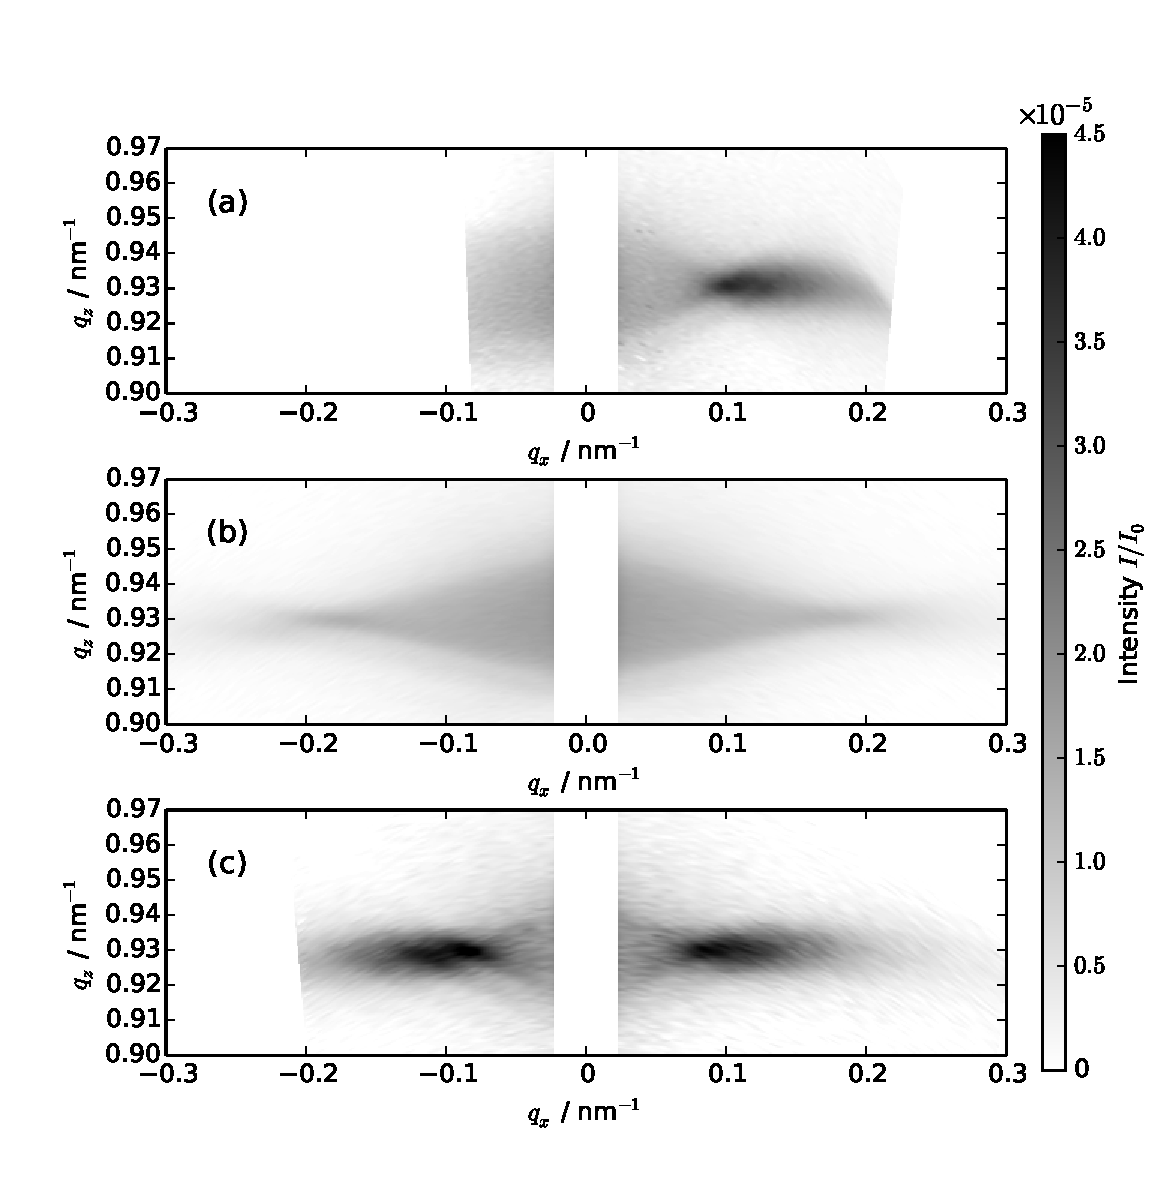
\includegraphics[width=
        0.8\textwidth]{measured_maps} \DIFaddendFL \caption{\DIFdelbeginFL \DIFdelFL{(a): }\DIFdelendFL Measured intensity map of a detector scan of a Mo/Si multilayer mirror at an angle of incidence $\alpha_i = 6.75^\circ$ \DIFdelbeginFL \DIFdelFL{. }\DIFdelendFL (\DIFdelbeginFL \DIFdelFL{b}\DIFdelendFL \DIFaddbeginFL \DIFaddFL{a}\DIFaddendFL ) \DIFdelbeginFL \DIFdelFL{:  Measured }\DIFdelendFL \DIFaddbeginFL \DIFaddFL{and  measured }\DIFaddendFL intensity \DIFdelbeginFL \DIFdelFL{map }\DIFdelendFL \DIFaddbeginFL \DIFaddFL{maps }\DIFaddendFL of the identical sample obtained through \DIFdelbeginFL \DIFdelFL{a }\DIFdelendFL rocking \DIFdelbeginFL \DIFdelFL{scan }\DIFdelendFL \DIFaddbeginFL \DIFaddFL{scans }\DIFaddendFL at an opening angle between detector and incident beam of $\Delta \Theta = 13.5^\circ$ \DIFaddbeginFL \DIFaddFL{(b) and $\Delta \Theta = 30^\circ$ (c)}\DIFaddendFL . The area close to the specular axis was excluded from this dataset due to its strong intensity compared to the diffuse scattering 
shown here. The access to the negative $q_x$-axis in (a) is limited due \DIFdelbeginFL \DIFdelFL{to technical and geometric limitations}\DIFdelendFL \DIFaddbeginFL \DIFaddFL{clipping of the incoming beam with the detector}\DIFaddendFL .} \label{fig:comparison} 
\end{figure*}
\subsection{Reciprocal Space Maps for Different Measurement Geometries} The reciprocal space maps in Fig.~\ref{fig:comparison} for the rocking scan (b) at an opening angle of $\Delta \Theta = 13.5^\circ$ \DIFaddbegin \DIFadd{and the rocking scan (c) at an opening angle of $\Delta \Theta = 30^\circ$ }\DIFaddend (corresponding to an angle of incidence of $\alpha_i = 6.75^\circ$ \DIFaddbegin \DIFadd{and $\alpha_i = 15.0^\circ$, respectively, }\DIFaddend in specular geometry) and for the detector scan with the angle of incidence $\alpha_i = 6.75^\circ$ clearly show different symmetries. We observe a strong enhancement in the off-specular scattering around $q_x\approx0.1$ nm$^{-1}$ (cf.~Fig.~\ref{fig:comparison}(a) \DIFaddbegin \DIFadd{and Fig.~\ref{fig:comparison}(c)}\DIFaddend ), which is not replicated on the negative $q_x$-axis \DIFaddbegin \DIFadd{in case of (a)}\DIFaddend . The rocking \DIFdelbegin \DIFdel{scan }\DIFdelend \DIFaddbegin \DIFadd{scans }\DIFaddend \ref{fig:comparison}(b) \DIFdelbegin \DIFdel{
is }\DIFdelend \DIFaddbegin \DIFadd{and \ref{fig:comparison}(c) are }\DIFaddend symmetric with respect to the specular axis at $q_x=0$, however, no enhanced scattering appears in \DIFdelbegin \DIFdel{this case}\DIFdelend \DIFaddbegin \DIFadd{(b)}\DIFaddend . The latter map shows a triangular-shaped intensity distribution for both the positive and 
negative $q_x$ range. A minimum in width with respect to the $q_z$ direction can be observed here around $q_x \approx \pm 0.2$ nm$^{-1}$. The triangular shape also appears for the 
positive $q_x$ range 
of the detector scan in Fig.~\ref{fig:comparison}(a), where the minimum in width coincides with the intensity maximum.


In Fig.~\ref{fig:BraggSheet_DetectorAndRocking}, the \DIFdelbegin \DIFdel{two }\DIFdelend \DIFaddbegin \DIFadd{three }\DIFaddend measurements shown above \DIFdelbegin \DIFdel{and a third rocking scan taken at an opening angle of $\Delta\Theta=30^\circ$ }\DIFdelend are compared by considering the intensity distribution along $q_z=0.93$ nm$^{-1}$, which corresponds to the momentum transfer at the multilayer resonance. The differences in the off-specular scattering are evident. 
\begin{figure}
	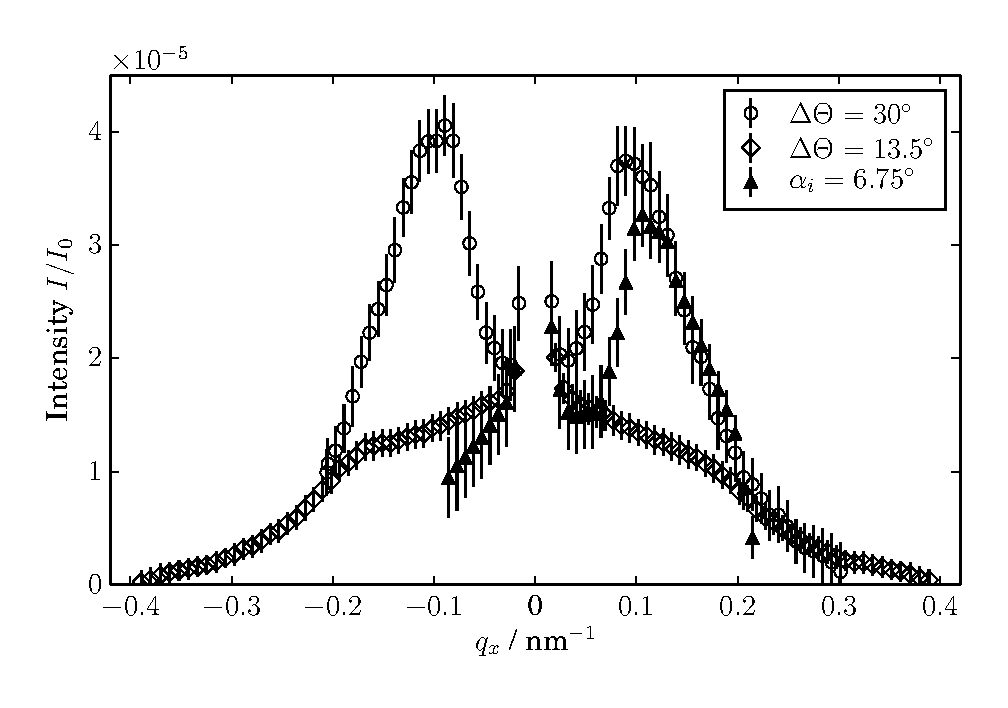
\includegraphics[width=0.5
	\textwidth]{BraggSheet_DetectorAndRocking} \caption{Averaged diffuse scattering intensity along $q_x$ in the interval  $q_z=(0.930 \pm 0.003$) nm$^{-1}$ corresponding to the resonance of the multilayer. The data shown are two rocking scan and one detector scan geometries (see text for details).} \label{fig:BraggSheet_DetectorAndRocking} 
\end{figure}

The measurement geometry dependence of the reciprocal space maps indicates that the intensity distributions cannot be the result of multilayer roughness properties alone, i.e. the power spectral density. Scattering intensities caused by roughness occur at identical positions in reciprocal space for any measurement geometry. In order to explain the observations shown here, the proper theoretical description of the diffuse scattering distributions is presented in the following section.

\section{Theoretical Background} \label{sec:theory} Our theoretical description of the diffuse EUV scattering from multilayers is based on the distorted-wave Born approximation (DWBA)~\cite{PhysRevB.49.10668,PhysRevB.47.15896}\DIFaddbegin \DIFadd{, widely used in the analysis of hard X-ray scattering}\DIFaddend . The DWBA is a perturbation theory in which the interfacial roughness is considered to be a small deviation from the ideal multilayer. This corresponds to a potential in the wave equation 
\begin{equation}
	(\Delta + K^2) |E(\mathbf{r})\rangle = V(\mathbf{r}) |E(\mathbf{r})\rangle\text{,} \label{eqn:wave_equation} 
\end{equation}
of $V(\mathbf{r}) = V_\text{id}(\mathbf{r}) + V_\text{r}(\mathbf{r})$ that can be separated into a strong part $V_\text{id}(\mathbf{r})$ for which an analytical solution exists and a small perturbation $V_\text{r}(\mathbf{r})$ describing the interfacial roughness. In case of a multilayer, we start from the \DIFdelbegin \DIFdel{fully }\DIFdelend dynamic calculation of the electric fields of a perfectly flat multilayer. The wave equation Eq.~\eqref{eqn:wave_equation} is solved by calculating the field amplitudes using a matrix formalism \cite{PrinciplesOfOptics}.

\DIFdelbegin \DIFdel{In order }\DIFdelend \DIFaddbegin 

\DIFadd{For the calculation of the specular reflectivity curve it is necessary }\DIFaddend to correct the \DIFdelbegin \DIFdel{specular }\DIFdelend field calculation for the interfacial roughness and \DIFdelbegin \DIFdel{interfacial diffusion, modified }\DIFdelend \DIFaddbegin \DIFadd{diffusion. Modified }\DIFaddend Fresnel coefficients according to N\'evot/Croece \cite{nevot_croece} assuming a Gaussian interface profile are used, 
\begin{align}
	r^{(j)} &= r_{id}^{(j)} \exp(-2 k_z^{(j)} k_z^{(j+1)} \sigma_j^2)\text{,} \DIFaddbegin \label{eqn:fresnel_r}\DIFaddend \\
	t^{(j)} &= t_{id}^{(j)} \exp((k_z^{(j)} - k_z^{(j+1)})^2 \sigma_j^2/2) \text{,} \DIFaddbegin \label{eqn:fresnel_t}
\DIFaddend \end{align}
where $r_{id}^{(j)}$ and $t_{id}^{(j)}$ are the Fresnel reflection and transmission coefficients, respectively, for the ideal  $j^\text{th}$ interface, $\sigma_j$ is the root mean square roughness (rms) and $k_z^{(j)}$ is the $z$-component of the incidence wave vector at the $j^\text{th}$ interface.

The diffuse scattering cross section is given by the covariance of the matrix element of the perturbation potential on the basis of the wave functions from the analytic solution for a given incidence and exit angle \cite{PhysRevB.38.2297,PhysRevB.49.10668} 
\begin{equation}
	\underset{\text{diffuse}}{\Big(\frac{d \sigma}{d \Omega}\Big)}= \text{Cov}(\langle E_{\text{id},1}| V_r|E_{\text{id},2}\rangle)\text{,} \label{eqn:incoherent_cross_section} 
\end{equation}
where $|E_{\text{id},i}\rangle\text{, }i =1,2$ are the solutions of the wave equation Eq.~\eqref{eqn:wave_equation} for the ideal multilayer and the given incidence and exit angles, respectively\DIFaddbegin \DIFadd{, calculated using the unmodified Fresnel coefficients $r_{id}^{(j)}$ and $t_{id}^{(j)}$ representing the perfectly flat multilayer}\DIFaddend . Since the roughness potential is non-zero only at the individual interfaces, Eq.~\eqref{eqn:incoherent_cross_section} can be decomposed into a sum over the matrix elements at each interface $j$. In the following, we use the small roughness $q_{z,j} \sigma_j \ll 1$ approximation which is valid for any high-quality multilayer mirror (cf. \cite{PhysRevB.53.6048} for the more general expression).

In the case of small reflectivity amplitudes, dynamic multiple reflections are often neglected and the dominant term in the decomposition is diffuse scattering of the transmitted fields at the roughness of each interface. The so-called semi-kinematic approximation \cite{PhysRevB.38.2297} yields an explicit expression for Eq.~\eqref{eqn:incoherent_cross_section} with
\begin{align}
                \overset{\text{semi-kinematic}}{\underset{\text{diffuse}}{\Big(\frac{d \sigma}{d \Omega}\Big)}} = &\frac{A \pi^2}{\lambda^4}\sum \limits_{j=1}^{N}\sum \limits_{i=1}^{N} \Big((n_j^2 - n_{j+1}^2)^* (n_i^2 - n_{i+1}^2) \nonumber \\ &\qquad\times T^{(1)*}_j T^{(2)*}_j T^{(1)}_i T^{(2)}_i S_{i j}(q_x)\Big)\text{,} \label{eqn:semi_kinematic_theory} 
\end{align}
where $A$ is the illuminated sample area, $\lambda$ the wavelength of the incident light and $n_j$ is the complex index of refraction of material $j$. The $T^{(1,2)}_j$ are defined as the amplitude of the transmitted field at the interface $j$ for the given exit angle (2) (represented as a time-inverted beam originating at the detector) and incidence angle (1). The total field at the $j$th interface is expressed in terms of the reflected field $E_r^{(j)}(z)$ propagating towards the vacuum and the transmitted field $E_t^{(j)}(z)$ propagating towards the substrate
\begin{align}
	E_t^{(j)}(z) &= T_{j} e^{i k_z^{(j)} z} \text{,} \\
	E_r^{(j)}(z) &= R_{j} e^{-i k_z^{(j)} z} \text{,} 
\end{align}
with $E_{id}^{(j)}(\mathbf{r}) = e^{i \mathbf{k_\parallel r_\parallel}} (E_t^{(j)}(z) + E_r^{(j)}(z))$ being the full solution of the wave equation Eq.~\eqref{eqn:wave_equation} for the ideal multilayer at the $j^\text{th}$ interface. $S_{ij}(q_x)$ is the structure factor describing the influence of the interfacial roughness on the diffuse scattering intensity \DIFdelbegin \DIFdel{. It has been shown }\DIFdelend \DIFaddbegin \DIFadd{defined through
}\begin{widetext}
\begin{align}
\DIFadd{S_{ij}(\vec{q}_\parallel; q_z^{(j)}, q_z^{(i)}) = \frac{\exp \Big[-((q_z^{(j)*})^{2} \sigma_j^2 + (q_z^{(i)})^{2} \sigma_i^2)/2\Big]}{q_z^{(j)*} q_z^{(i)}} \int d^2 \vec{X} \Big(\exp [q_z^{(j)*} q_z^{(i)} C_{ij}(\vec{X})]-1\Big) \exp(i \vec{q}_\parallel \cdot \vec{X}) \text{,} }\label{eqn:full_structure_factor}
\end{align}
\end{widetext}
\DIFadd{where $q_z^{(i)}$ is the $z$-component of the scattering vector $\vec{q}$ at the $i$th interface, $\vec{X} = \vec{x} - \vec{x}'$ is the lateral distance vector and $C_{ij}(\vec{x}-\vec{x}') = \langle h_i(\vec{x}) h_j(\vec{x}') \rangle$ is the correlation function of the interface profiles $h(\vec{x})$ of the interfaces $i$ and $j$ }\DIFaddend \cite{PhysRevB.51.5297,PhysRevB.53.6048}\DIFdelbegin \DIFdel{that }\DIFdelend \DIFaddbegin \DIFadd{. In case of the small roughness approximation, }\begin{align}
\DIFadd{\frac{\exp \Big[-((q_z^{(j)*})^2 \sigma_j^2 + (q_z^{(i)})^{2} \sigma_i^2)/2\Big]}{q_z^{(j)*} q_z^{(i)}} \approx \frac{1}{q_z^{(j)*} q_z^{(i)}}
}\end{align}
\DIFadd{and $\exp [q_z^{(j)*} q_z^{(i)} C_{ij}(\vec{X})]-1 \approx q_z^{(j)*} q_z^{(i)} C_{ij}(\vec{X})$ apply and Eq.~}\eqref{eqn:full_structure_factor} \DIFadd{reduces to
}\begin{align}
\DIFadd{S_{ij}(\vec{q}_\parallel) \approx \int d^2 \vec{X} C_{ij}(\vec{X}) \exp(i \vec{q}_\parallel \cdot \vec{X}) \text{.} }\label{eqn:reduced_structure_factor}
\end{align}
\DIFadd{$S_{ij}(\vec{q}_\parallel)$ is, thus, the Fourier transform of the correlation function $C_{ij}(\vec{X})$. In case of co-planar scattering furthermore $\vec{q}_\parallel \equiv \vec{q}_x$.
Assuming identical growth for the individual layers, i.e.~a material independent propagation of roughness along the $z$-direction, }\DIFaddend $S_{ij}(q_x)$ can be expressed in terms of the lateral power spectral density (PSD) \DIFaddbegin \DIFadd{$C_{i}(q_x)$ }\DIFaddend and a vertical \DIFdelbegin \DIFdel{correlation function. 
}\DIFdelend \DIFaddbegin \DIFadd{replication factor $c_{ij}^{\perp}(q_x)$ }\cite{spiller1993multilayer}\DIFadd{,
}\DIFaddend \begin{equation}
	S_{ij}(q_x) = c_{ij}^{\perp}(q_x) C_{\text{max}(i,j)}(q_x)\text{.} \DIFaddbegin \label{eqn:factorized_structure_factor}
\DIFaddend \end{equation}

\DIFdelbegin \DIFdel{Several power spectral density functions }\DIFdelend \DIFaddbegin \DIFadd{Other PSD functions based on different models of lateral interface roughness correlation }\DIFaddend have been proposed\DIFdelbegin \DIFdel{. }\DIFdelend \DIFaddbegin \DIFadd{, e.g.~by Sinha et al.~}\cite{PhysRevB.38.2297}\DIFadd{. We follow the approach by de Boehr et al.~}\cite{deBoerLateralCorrelation,PhysRevB.51.5297} \DIFadd{for fractal interface roughness, where the lateral correlation function of the $i$th interface is given by
}\begin{align}
\DIFadd{\tilde{C}_i(\vec{X}) = P_i \xi_\parallel^{H_i} |\vec{X}|^{H_i} K_{H_i}\Big(|\vec{X}|/\xi_\parallel\Big) \text{.} }\label{eqn:lateral_correlation_function}
\end{align}
\DIFadd{$H_i$ is the Hurst factor providing a measure for the jaggedness of the interface }\cite{PhysRevB.38.2297}\DIFadd{, $K_{H_i}$ are the modified Bessel functions of the order $H_i$, $\xi_\parallel$ is a lateral correlation length and
}\begin{align}
\DIFadd{P_i = \frac{\sigma_i^2}{\xi_\parallel^{H_i-1} 2^{H_i-1} \Gamma(1+H_i)/H_i}\text{.}
}\end{align}

\DIFaddend Our goal is to determine a single average power spectral density. We thus do not distinguish between individual interfaces in the model and assume an identical roughness \DIFdel{profile} \DIFadd{properties} for all interfaces. Hence $\sigma_j = \sigma$\DIFaddbegin \DIFadd{, $H_j = H$ }\DIFaddend and $C_{\text{max}(i,j)}(q_x) = C(q_x)$. \DIFdelbegin \DIFdel{In our case, $C(q_x)$ is represented by the closed analytical form
proposed by de Boehr }%DIFDELCMD < \cite{PhysRevB.53.6048,PhysRevB.51.5297}
%DIFDELCMD < %%%
\DIFdelend \DIFaddbegin \DIFadd{The PSD is given by the Fourier transform of Eq.~}\eqref{eqn:lateral_correlation_function} \DIFadd{with respect to $q_x$, which yields the closed analytic form
}\DIFaddend \begin{equation}
	C(q_x) = \frac{4 \pi H \sigma^2 \xi_\parallel^2}{(1+|q_x|^2\xi_\parallel^2)^{1+H}} \text{\DIFdelbegin \DIFdel{,}\DIFdelend \DIFaddbegin \DIFadd{.}\DIFaddend } \label{eqn:psd} 
\end{equation}

\DIFdelbegin \DIFdel{where $\xi_\parallel$ is a lateral correlation length and $H$ is the Hurst factor providing a measure for the jaggedness of the interface }
\DIFdel{. This approach is not limited to this particular representation of the power spectral density. Other models are equally applicable here and can be found elsewhere in the literature (e.g.~}\DIFdel{).}\DIFdelend 


The high degree of thickness stability for well-defined multilayers as is necessary for high-performance mirrors implies a high degree of vertical correlation of individual interfaces \DIFdelbegin \DIFdel{. We thus consider a simple correlation function of roughness with the vertical correlation length $\xi_\perp$ for the description of the diffuse scattering 
}\DIFdel{$c_{ij}^{\perp}$}
\DIFdelend \DIFaddbegin \DIFadd{roughness throughout the stack. In order to derive the replication factor in Eq.~}\eqref{eqn:factorized_structure_factor}\DIFadd{, we follow Stearns et al.~}\cite{stearns:4286}\DIFadd{. In this model, the evolution of the surface roughness $w(x,y)$ during the growth of a single layer is described by the Langevin equation. In its Fourier transformed form, 
}\begin{align}
\DIFadd{\frac{\partial w(f)}{\partial t} = - 4 \pi^2 v f^2 w(f) + \frac{\partial \eta(f)}{\partial t} \text{,} }\label{eqn:langevin}
\end{align}
\DIFadd{where $v$ is a diffusion-like parameter, $\eta(f)$ is random noise normalized to the layer thickness and $w(f)$ describes the roughness evolution in dependence of the spacial frequency $f$. The roughness evolution during the growth of a single layer of a specific material can then be evaluated by discritizing Eq.~}\eqref{eqn:langevin} \DIFadd{for the successive deposition of material of thickness $\delta d$
}\begin{align}
\DIFadd{w_i(f) = c_\perp(f;\delta d) w_{i-1}(f) + \eta(f) \text{,}
}\end{align}
\DIFadd{where $c_\perp(f;\delta d)$ is the replication factor of roughness for a single deposition. In the limit of repeated infinitesimal depositions until the full $n$th layer of thickness $d_n$ is grown, $c_\perp(f,d_n)$ can be evaluated to be }\cite{spiller1993multilayer}
\begin{align}
    \DIFadd{c_\perp(f,d_n) }&\DIFadd{= \exp(-4\pi^2 f^2 v }\,\DIFadd{d_n) }\nonumber \\
                   &\DIFadd{= \exp(-q_x^2 v }\,\DIFadd{d_n)\text{,}
}\end{align}
\DIFadd{with $q_x^2 = 4 \pi^2 f^2$. Assuming identical diffusionlike behavior $v$ for all materials of a multilayer and defining $\xi_\perp(q_x) = 1/(v q_x^2)$, the replication factor in Eq.~}\eqref{eqn:factorized_structure_factor} \DIFadd{is given by
}\begin{align}
c_{ij}^\perp (q_x) =  \exp \Bigg (-\sum \limits_{n = \text{min}(i,j)}^{\text{max}(i,j) -1\DIFaddend }d_n/\xi_\perp  \DIFaddbegin \DIFadd{(q_x) }\Bigg)\text{.}
\end{align}
\DIFadd{Here, $\xi_\perp(q_x)$ can be interpreted as a frequency dependent vertical correlation length, describing the distance perpendicular to the stack until the replication factor decreased to $1/e$.}

\DIFadd{Gullikson et al.~}\cite{PhysRevB.59.13273} \DIFadd{observed that the direction of the vertical replication of roughness can be tilted with respect to the surface normal. This leads to tilted Bragg planes requiring a coordinate transformation in reciprocal space to account for the tilt angle $\beta$ according to
}\begin{align}
\DIFadd{\overline{q}_z = q_z - q_x \tan \beta}\DIFaddend \text{.}
\DIFdelbegin %DIFDELCMD < \end{equation}
\end{align}%DIFAUXCMD
%DIFDELCMD < 
%%%
\begin{align}%DIFAUXCMD
\DIFdelend \DIFaddbegin \end{align}
\DIFadd{Since the vertical scattering vector components enter the calculations through the Fresnel coefficients $r_{id}^{(j)}$ and $t_{id}^{(j)}$, an additional factor enters the calculation of Eq.~}\eqref{eqn:factorized_structure_factor} \DIFadd{through substitution by
}\begin{align}
\DIFadd{\overline{S_{ij}}(q_x) = \exp\Big(-i q_x \tan \beta (z_i-z_j)\Big)  S_{ij}(q_x) \text{,} }\label{eqn:tilt_correction}
\end{align}
\DIFadd{where $z_i$ is the $z$-position of the $i$th interface.}\DIFaddend 

So far, multiple reflections at the interfaces have been ignored (semi-kinematic approximation). However, in the case of high-reflectance multilayer mirrors, this might not be valid. In order to include \DIFdelbegin \DIFdel{these }\DIFdelend \DIFaddbegin \DIFadd{first order multiple reflections, i.e.~single reflection and transmission processes before and after the diffuse scattering event, }\DIFaddend in the theoretical treatment\DIFdelbegin \DIFdel{for comparison}\DIFdelend , the reflected fields need to be included in Eq.~\eqref{eqn:incoherent_cross_section}. The explicit expression considering dynamic multiple reflections within the layer is given by
\begin{widetext}
    \begin{align}
        \DIFdelbegin %DIFDELCMD < \overset{\text{fully dynamic}}{\underset{\text{diffuse}}{\Big(\frac{d \sigma}{d \Omega}\Big)}} %%%
\DIFdelend \DIFaddbegin \overset{\text{dynamic}}{\underset{\text{diffuse}}{\Big(\frac{d \sigma}{d \Omega}\Big)}} \DIFaddend = &\Bigg[\frac{A \pi^2}{\lambda^4}\sum \limits_{j=1}^{N}\sum \limits_{i=1}^{N} (n_j^2 - n_{j+1}^2)^* (n_i^2 - n_{i+1}^2)\Big( (T^{(1)}_j + R^{(1)}_j)^* (T^{(2)}_j + R^{(2)}_j)^* \nonumber \\ &\qquad\times(T^{(1)}_i + R^{(1)}_i) (T^{(2)}_i + R^{(2)}_i) \Big) c_\perp^{i j}\Bigg]\,\, C(q_x) \text{,} \label{eqn:multilayer_enhancement_factor}
    \end{align}
\end{widetext}
where $R^{(1,2)}_j$ are the reflected field amplitude at interface $j$ for the given incidence angle (1) and exit angle (2), the latter again in a time-inverted representation of a beam originating at the detector.


\section{Numerical Simulations} \label{sec:numerical_simulations} We have applied the theory above to the multilayer in our experiments. In order to obtain a model for the layer thicknesses in our multilayer, we measured the reflectivity of the sample in dependence on the wavelength. The recorded curve was fitted using the \DIFdelbegin \DIFdel{\emph{IMD} software }%DIFDELCMD < \cite{windt1998imd}%%%
\DIFdel{.}\DIFdelend \DIFaddbegin \DIFadd{numerical calculation of the reflectivity curve based on the specular fields including the modified Fresnel coefficients in Eq.~}\eqref{eqn:fresnel_r} \DIFadd{and Eq.~}\eqref{eqn:fresnel_t}\DIFadd{. }\DIFaddend The resulting fit parameters were, then, further used to model the multilayer in the numerical simulations below. The \DIFdelbegin \DIFdel{individual }\DIFdelend \DIFaddbegin \DIFadd{fit of the reflectivity curve was later simultaneously optimized during the fit of the diffuse scattering in order to correct for the change in the mean roughness $\sigma$. The final }\DIFaddend thicknesses in the stack were fitted to \DIFdelbegin \DIFdel{$d_\text{Mo} = 2.025$ nm, $d_\text{B$_4$C} = 1.327$ nm, $d_\text{Si} = 3.041$ nm and $d_\text{C} = 0.582$ nm}\DIFdelend \DIFaddbegin \DIFadd{ $d_\text{Mo} = 2.0181$ nm, $d_\text{B$_4$C} = 1.3215$ nm, $d_\text{Si} = 3.0388$ nm and $d_\text{C} = 0.5858$ nm}\DIFaddend. The distorted-
wave Born approximation was implemented in the \emph{Python} programming language using a highly parallel algorithm.

\subsection{Dynamic Contributions to the Diffuse Scattering} \label{sec:dynamic_contributions} 
In order to determine the contribution of dynamic multiple reflections within the stack, we compared the semi-kinematic approximation in Eq.~\eqref{eqn:semi_kinematic_theory} with the \DIFdelbegin \DIFdel{fully }\DIFdelend dynamic calculations in Eq.~\eqref{eqn:multilayer_enhancement_factor}. For this comparison, we simulated a rocking scan at an opening angle of $\Delta \Theta = 30^\circ$ \DIFdelbegin \footnote{\DIFdel{The roughness properties for these simulations were determined following the procedure described in Sec.~\ref{sec:determination_of_the_psd}.}} %DIFAUXCMD
\addtocounter{footnote}{-1}%DIFAUXCMD
\DIFdelend and compared the simulations with the measured data. \DIFaddbegin \DIFadd{The roughness properties for these simulations were determined following the procedure described below in Sec.~\ref{sec:determination_of_the_psd} including a discussion on the influence of the parameters, specifically $\xi_\perp(q_x)$, on these vertical line cuts.}\DIFaddend 

A quantitative comparison of the dynamic contribution to the total scattering intensity in our measurements is shown in Fig.~\ref{fig:Comparison_full_semi} as a line cut along $q_z$ at $q_x=0.05$ nm$^{-1}$. The \DIFdelbegin \DIFdel{fully }\DIFdelend dynamic calculation yields excellent agreement with the measured data. The results show distinct differences with an increase up to 100\% of the scattered intensity close to the multilayer resonance at $q_z=0.93$ nm$^{-1}$ compared to the semi-kinematic calculation. Hence dynamic contributions are dominant in the vicinity of the Bragg resonance. 
\begin{figure}
        \DIFdelbeginFL %DIFDELCMD < \includegraphics[width=0.5
%DIFDELCMD <         \textwidth]{Comparison_full_semi} %%%
\DIFdelendFL \DIFaddbeginFL 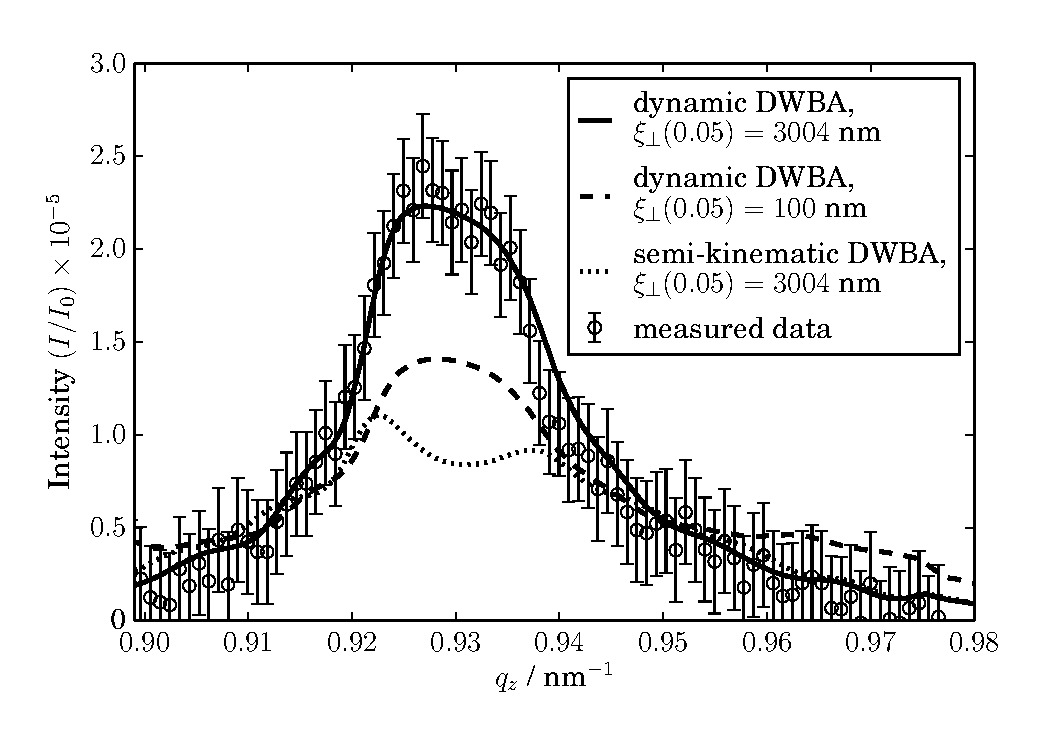
\includegraphics[width=0.5
        \textwidth]{qz_kinematic_vs_dynamic_100nm} \DIFaddendFL \caption{Scattering intensity along $q_z$ for $q_x=0.05$ nm$^{-1}$ for the \DIFdelbeginFL \DIFdelFL{full }\DIFdelendFL dynamic and semi-kinematic calculations for a rocking scan at $\Delta\Theta=30^\circ$ \DIFaddbeginFL \DIFaddFL{in comparison to the measured data}\DIFaddendFL .} \label{fig:Comparison_full_semi} 
\end{figure}

To evaluate the contribution of multiple reflections due to the subsidiary maxima, Fig.~\ref{fig:kiessig_like_peak} shows the intensity distribution along $q_x$ at $q_z=0.93$ nm$^{-1}$.  These maxima are caused by interference of the reflections from the top surface of the multilayer stack and the substrate interface (Kiessig fringes) \cite{kiessig1931}.
\begin{figure}
        \DIFdelbeginFL %DIFDELCMD < \includegraphics[width=0.5
%DIFDELCMD <         \textwidth]{kiessig_like_peak} %%%
\DIFdelendFL \DIFaddbeginFL 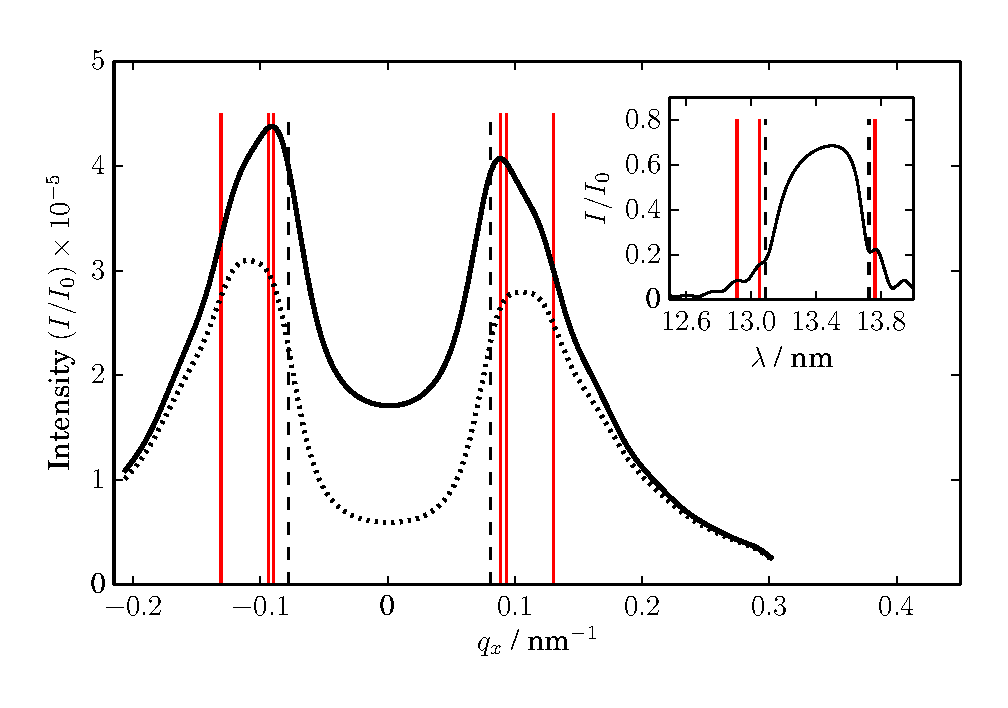
\includegraphics[width=0.5
        \textwidth]{qx_kinematic_vs_dynamic} \DIFaddendFL \caption{Scattering intensity distribution at $q_z=0.93$ nm$^{-1}$. The solid line shows the result of the \DIFdelbeginFL \DIFdelFL{fully }\DIFdelendFL dynamic calculation for a rocking scan with an opening angle of $\Delta\Theta=30^\circ$. The dashed line represents the calculation applying the semi-kinematic approximation, ignoring any multiple reflections within the multilayer. The dashed vertical lines are the limits of the main Bragg peak, while the red solid vertical lines show the position of dynamic contributions of the Kiessig fringes close to the main maximum. Each Kiessig fringe marked in the inset appears for the corresponding positive and negative $q_x$ value. The strong intensity at $q_x\approx0.1$ nm$^{-1}$ results from the overlap of the dynamic maxima of two different Kiessig fringes (see text).} \label{fig:kiessig_like_peak} 
\end{figure}
The solid line corresponds to the \DIFdelbegin \DIFdel{fully }\DIFdelend dynamic theory, while the dotted line is the result of the semi-kinematic calculation. The dashed vertical lines indicate the limits of the main Bragg peak. These positions are defined through the first minimum on each side of the reflectivity peak (cf.~inset in Fig.~\ref{fig:kiessig_like_peak}). The vertical red lines show the position of multiple reflections due to Kiessig fringes close to the main resonance. Again, the corresponding positions in the specular reflectivity measurement are shown in the inset. Each of the marked fringes appears on the negative and positive $q_x$-axis in the main plot. This is caused by the incidence and exit angle, respectively, being at the resonance angle of the various Kiessig maxima in the reflectivity curve. Thus, a strong increase with respect to the semi-kinematic approximation is observed. The position of the dynamic contribution from the first 
Kiessig fringes on either side of the main resonance exhibits a pronounced maximum in the diffuse scattering. These fringes contribute most due to their high overall relative 
intensity compared with the fringes further away from the reflectivity maximum. In addition, the position in reciprocal space coincides with the first two Kiessig fringes marked on either side of the main maximum. This effect of dynamic maxima is similar to the observation of Bragg-like peaks in grazing incidence geometry \cite{PhysRevB.52.16369}, but it is caused by the subsidiary maxima instead. Consequently, we name this enhancement ``Kiessig-like peaks''. The contribution by the main Bragg resonance similar to the observations in Fig.~\ref{fig:Comparison_full_semi} amounts to approximately 100\% at $q_x=0$.

\subsection{Multilayer Enhancement Factor} \label{sec:multilayer_contribution}
\DIFdelbegin \DIFdel{Apart from the purely dynamic maxima, which constitute a contribution to the geometry-dependent diffuse scattering, intrinsic properties of scattering from multilayer mirrors cause a strong enhancement. }\DIFdelend The total contribution of the multilayer \DIFaddbegin \DIFadd{top the diffuse scattering}\DIFaddend , independent of lateral interface roughness properties, \DIFdelbegin \DIFdel{was analyzed in our model by considering only }\DIFdelend \DIFaddbegin \DIFadd{is described by }\DIFaddend the sum in the square brackets of Eq.~\eqref{eqn:multilayer_enhancement_factor} as a prefactor to the power spectral density $C(q_x)$. It \DIFdelbegin \DIFdel{contains all the information on the scattering behavior from multilayers}\DIFdelend \DIFaddbegin \DIFadd{describes the modulation of the scattering intensity due to the multilayer nature of the scattering structure}\DIFaddend , independent of the interface roughness. We thus consider it as a ``relative multilayer enhancement factor''. The 
result of the calculations based on the layer model of our multilayer sample is shown in Fig.~\ref{fig:MultilayerInfluence} for one detector and two rocking scan configurations. The vertical correlation length \DIFdelbegin \DIFdel{is $\xi_\perp=400$ nm}\DIFdelend \DIFaddbegin \DIFadd{for this specific multilayer mirror is $\xi_\perp(q_x)=7.5/q_x^2$ nm$^{-1}$ }\DIFaddend as expected for a high-reflectance mirror, where $\xi_\perp$ 
\DIFdelbegin \DIFdel{approaches }\DIFdelend \DIFaddbegin \DIFadd{exceeds }\DIFaddend the total thickness $D$ of the entire stack \DIFaddbegin \DIFadd{for $|q_x| < 0.12$ nm$^{-1}$}\DIFaddend . The method for the extraction of the vertical correlation length from the measured data is \DIFdelbegin \DIFdel{presented }\DIFdelend \DIFaddbegin \DIFadd{discussed }\DIFaddend in Sec.~\ref{sec:determination_of_the_psd}. The multilayer enhancement factor was normalized with respect to $q_x=0$, i.e. the calculated diffuse scattering contribution on the specular axis. 
\begin{figure}
	\DIFdelbeginFL %DIFDELCMD < \includegraphics[width=0.5
%DIFDELCMD < 	\textwidth]{Multilayer_influence} %%%
\DIFdelendFL \DIFaddbeginFL 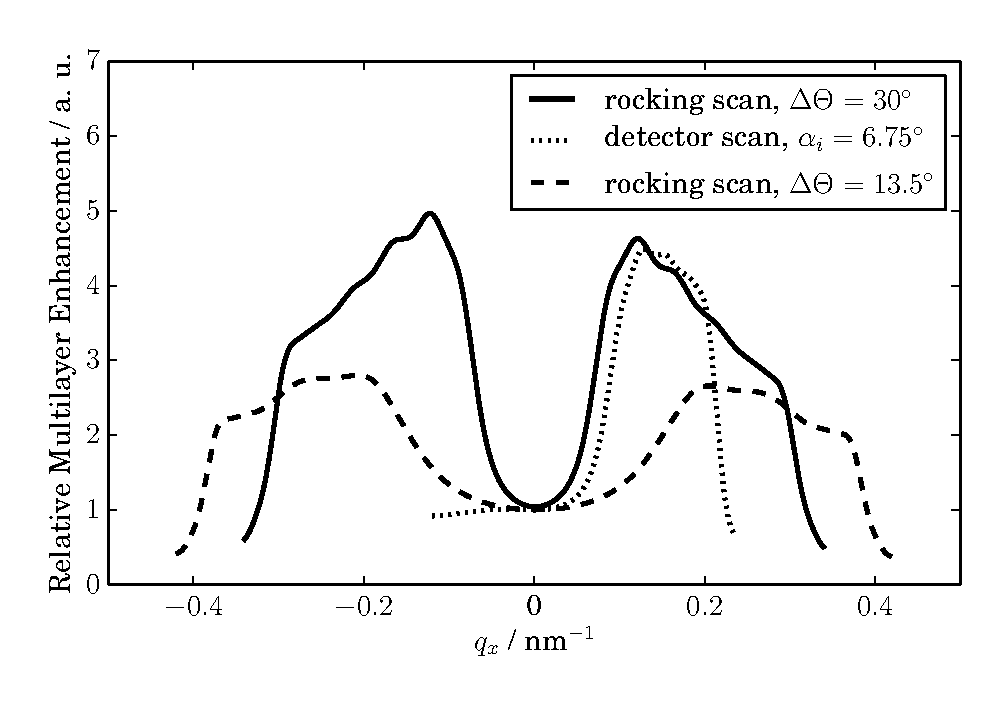
\includegraphics[width=0.5
	\textwidth]{MEF} \DIFaddendFL \caption{Enhancement factor due to the specific properties of multilayer reflectivity for three different measurement geometries. The simulations shown here were normalized with respect to the diffuse contribution to the specular reflectivity at $q_x=0$.} \label{fig:MultilayerInfluence} 
\end{figure}

The results clearly show that diffuse scattering from multilayers at near-normal incidence exhibit strong enhancement due to the intrinsically limited bandpass of reflectivity of multilayers. If both the incidence and exit angle is out of the Bragg resonance, the higher penetration depth of the multilayer causes an increase in the number of interfaces contributing to the diffuse scattering intensity. Thus higher total scattering is observed. The Kiessig fringes cause modulations in the enhancement factor increased by the purely dynamic processes described in Sec.~\ref{sec:dynamic_contributions}.

\begin{figure*}
        \DIFdelbeginFL %DIFDELCMD < \includegraphics[width=
%DIFDELCMD <         \textwidth]{Comparison_with_theory} %%%
\DIFdelendFL \DIFaddbeginFL 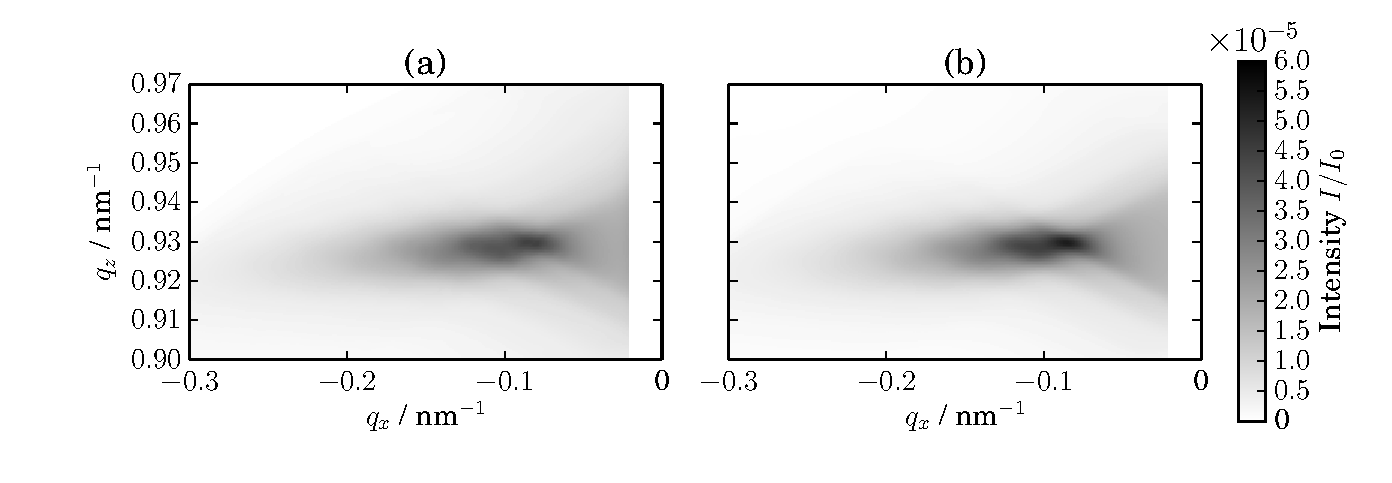
\includegraphics[width=
        \textwidth]{simulation_vs_measurement} \DIFaddendFL \caption{Measured (a) and simulated (b) reciprocal space maps for a rocking scan at an opening angle of $\Delta\Theta=30^\circ$ with the roughness parameters determined in Sec.~\ref{sec:determination_of_the_psd}.} \label{fig:comparisonWithTheory} 
\end{figure*}

\subsection{Reconstruction of the Power Spectral Density} \label{sec:determination_of_the_psd} In order to extract roughness properties from the off-specular measurements shown above, a correction for the influence of the multilayer as discussed in Sec.~\ref{sec:multilayer_contribution} is required. The scattering intensity after division by the multilayer enhancement factor represents the power spectral density of roughness. The measured PSDs are shown in Fig.~\ref{fig:PSDs_linear} for all three experiments. The excellent agreement with each other within the uncertainty margin confirms the validity and necessity of the \DIFdelbegin \DIFdel{fully }\DIFdelend dynamic theory to model the diffuse scattering from the multilayer. The reconstruction of the parameters of the power spectral density in Eq.~\eqref{eqn:psd} can be done by considering the overall intensity as well as the asymptotic behavior \cite{PhysRevB.54.5860} of the measured data in Fig.~\ref{fig:PSDs_linear}.

The numerical simulations show a strong sensitivity with respect to the mean roughness parameter $\sigma$ through the total portion of diffusely scattered light. As expected for a high-reflectance mirror, we obtained a small roughness value of \DIFdelbegin \DIFdel{$\sigma = 0.21$ }\DIFdelend \DIFaddbegin \DIFadd{$\sigma = 0.2$ }\DIFaddend nm.
\begin{figure}
	\DIFdelbeginFL %DIFDELCMD < \includegraphics[width=0.5
%DIFDELCMD < 	\textwidth]{PSDs_linear} %%%
\DIFdelendFL \DIFaddbeginFL 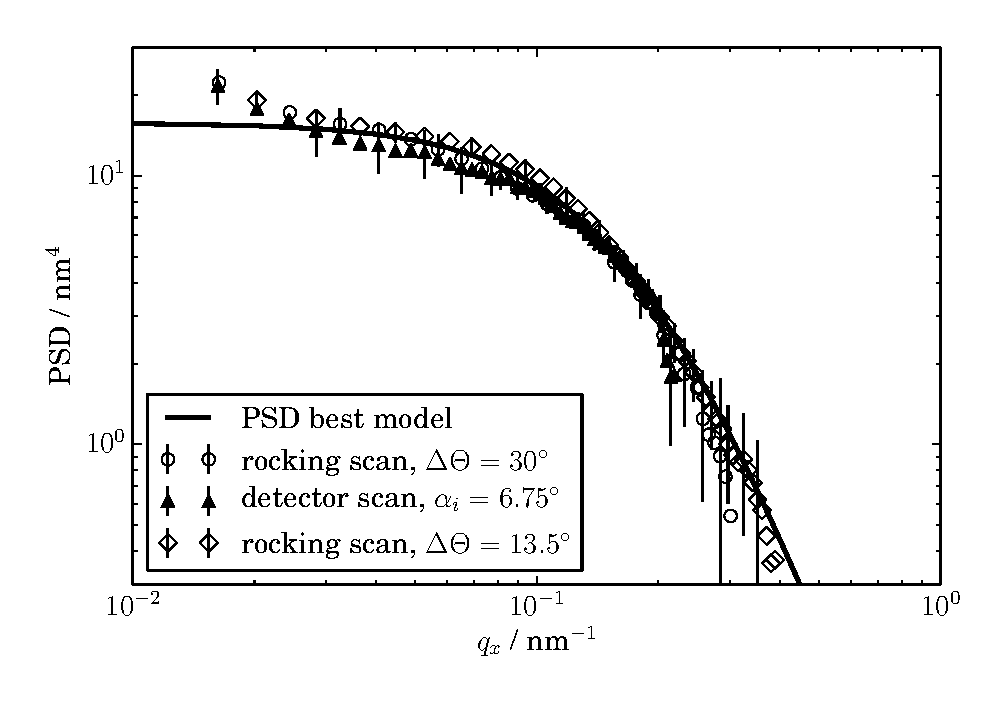
\includegraphics[width=0.5
	\textwidth]{PSD_zoomed} \DIFaddendFL \caption{Diffuse scattering intensity corrected for the multilayer enhancement factor \DIFaddbeginFL \DIFaddFL{considering a tilt angle of $\beta=-1^{\circ}$ according to Eq}\DIFaddendFL .\DIFaddbeginFL \DIFaddFL{~}\eqref{eqn:tilt_correction}\DIFaddFL{. }\DIFaddendFL The black solid line corresponds to a power spectral density with \DIFdelbeginFL \DIFdelFL{$\xi_\parallel=6.5$ }\DIFdelendFL \DIFaddbeginFL \DIFaddFL{$\xi_\parallel=5.6$ }\DIFaddendFL nm, $H=1.0$, \DIFdelbeginFL \DIFdelFL{$\sigma=0.21$ }\DIFdelendFL \DIFaddbeginFL \DIFaddFL{$\sigma=0.2$ }\DIFaddendFL nm and a vertical correlation length of \DIFdelbeginFL \DIFdelFL{$\xi_\perp=400$ }\DIFdelendFL \DIFaddbeginFL \DIFaddFL{$\xi_\perp(q_x)=7.5/q_x^2$ }\DIFaddendFL nm\DIFaddbeginFL \DIFaddFL{$^{-1}$}\DIFaddendFL .} \label{fig:PSDs_linear} 
\end{figure}

It follows from the definition of the PSD in Eq.~\eqref{eqn:psd} that the lateral correlation length $\xi_\parallel$ defines a cut-off for the spatial frequencies contributing \DIFadd{to} the off-specular scattering. We performed several simulations to compare the simulated intensity profile with the cut-off frequency observed in the measured data. A correlation length of \DIFdelbegin \DIFdel{$\xi_\parallel=6.5$ }\DIFdelend \DIFaddbegin \DIFadd{$\xi_\parallel=5.6$ }\DIFaddend nm was obtained following this method. The fractal nature of the interfaces was analyzed by varying the Hurst parameter $H$. The asymptotic behavior of the power spectral density for $q_x>10^{-1}$\DIFaddbegin \DIFadd{~}\DIFaddend nm$^{-1}$ for the multilayer sample measured yields a Hurst factor of $H=1.0$, which corresponds to a smooth roughness profile \cite{PhysRevB.38.2297}. By following this procedure, measurements of power spectral densities are possible, independent of the measurement geometry.

For a full characterization of the multilayer, the determination of the vertical correlation length remains. This parameter is also accessible through the two-dimensional reciprocal space maps. It has been observed elsewhere that the vertical correlation of the interfacial roughness leads to resonant diffuse scattering (``Bragg sheets'')~\cite{PhysRevB.49.10668}. The width of these sheets with respect to the $q_z$-axis provides a measure for the vertical correlation lengths, e.g.~in GISAXS \cite{Siffalovic200919}. We observe a similar dependence of the scattering intensity close to the Bragg resonance along the vertical axis \DIFdelbegin \DIFdel{. We performed several numerical simulations varying the vertical correlation length $\xi_\perp$.  Fig.~5 shows the intensity distribution along that axis for two different correlation lengths (solid and dashed lines)}\DIFdelend \DIFaddbegin \DIFadd{(cf.~ Fig.~\ref{fig:Comparison_full_semi}) with a reduction of the scattering intensity at the resonance for small correlation length but a higher relative scattering intensity far off resonance (cf. $q_z>0.95$ nm$^{-1}$ in Fig.~\ref{fig:Comparison_full_semi})}\DIFaddend. We varied the 
vertical correlation length $\xi_\perp(q_x)$ and fitted several vertical cuts of the reciprocal space map simultaneously with the PSD determination\DIFaddend . The best model for our sample yields a high vertical correlation length of \DIFdelbegin \DIFdel{$400$ nm}\DIFdelend \DIFaddbegin \DIFadd{$\xi_\perp(q_x)=7.5/q_x^2$ nm$^{-1}$, }\DIFaddend as expected for high-reflectance mirrors\DIFaddbegin \DIFadd{, at a tilt angle of $\beta=-1^\circ$ of the Bragg plane}\DIFaddend . 
This correlation length \DIFdelbegin \DIFdel{approaches }\DIFdelend \DIFaddbegin \DIFadd{exceeds }\DIFaddend the total thickness of the multilayer coating \DIFaddbegin \DIFadd{up to $|q_x|<0.13$ nm$^{-1}$ }\DIFaddend and thus indicates (almost) full \DIFdelbegin \DIFdel{correlation of all interfaces}\DIFdelend \DIFaddbegin \DIFadd{replication of roughness throughout all interfaces for the specified spacial frequencies}\DIFaddend .

By combining the findings for the properties of roughness in the power spectral density and the multilayer enhancement factor determined by the layer structure of the multilayer, we are able to fully reconstruct the measured intensity distribution for all geometries. The simulated reciprocal space map for a rocking scan with an opening angle of $\Delta\Theta = 30^\circ$ based on the parameters determined in the previous analysis is shown in Fig.~\ref{fig:comparisonWithTheory}(b). The calculation is in excellent agreement with the measured reciprocal space map in Fig.~\ref{fig:comparisonWithTheory}(a). 


\section{Conclusions} We have applied near-normal incidence diffuse scattering in the EUV spectral range to analyze the interfacial roughness of Mo/Si multilayers. At-wavelength reciprocal space maps in the vicinity of the main Bragg resonance of the multilayer were recorded for the first time via angle and wavelength resolved scatterometry. We observed intensity enhancements in the off-specular scattering. Experiments in different geometries revealed a dependence of the off-specular scattered intensity on the measurement geometry.

Numerical simulations based on the distorted-wave Born approximation (DWBA) have been performed. The comparison of semi-kinematic simulations with \DIFdelbegin \DIFdel{fully }\DIFdelend dynamic calculations show that dynamic effects, i.e.~multiple reflections at the interfaces, cannot be neglected. The semi-kinematic approach is invalid when either incidence or exit angle fulfill the Bragg condition. In addition, dynamic multiple reflections caused by increased reflectivity due to the Kiessig fringes close to the main Bragg resonance contribute significantly to the off-specular scattering distribution. The simulations show that the limited bandpass reflection property of the multilayer causes the geometry-dependent diffuse scattering in conjunction with the dynamic maxima.

Therefore, in the determination of the interface morphology from co-planar reciprocal space maps a multilayer enhancement factor has to be considered to extract the power spectral density (PSD). We have applied our model to two different measurement geometries with two different angles of incidence for the specular case. Together with the multilayer composition determined from modeled specular reflectivity curves \DIFdelbegin \DIFdel{(XRR) }\DIFdelend rigorous simulations of the diffuse scattering intensity caused by the multilayer were possible, in excellent agreement with the measured data. The average lateral power spectral density could then be extracted with regard to the multilayer enhancement factor equivalently for any measurement geometry. In addition, measurements along the $q_z$ direction provide information on the vertical correlation of interfaces, i.e.~the determination of the vertical correlation length. 

In conclusion, \DIFdelbegin \DIFdel{this }\DIFdelend \DIFaddbegin \DIFadd{the consideration of the dynamic effects in the DWBA }\DIFaddend allows the characterization of the multilayer with respect to its roughness properties. The diffuse scattering measurements corrected for the multilayer enhancement factor provide a \DIFdelbegin \DIFdel{direct }\DIFdelend measure of the power spectral density. Thus, this method is not restricted to the specific representation of the power spectral density used in our model. Alternative power spectral density models have been discussed in the literature \cite{PhysRevB.38.2297, PhysRevB.48.2873} and are equivalently applicable in the numerical simulations.



%\section*{Acknowledgments} TBD

%merlin.mbs apsrev4-1.bst 2010-07-25 4.21a (PWD, AO, DPC) hacked
%Control: key (0)
%Control: author (8) initials jnrlst
%Control: editor formatted (1) identically to author
%Control: production of article title (-1) disabled
%Control: page (0) single
%Control: year (1) truncated
%Control: production of eprint (0) enabled

\bibliographystyle{osajnl}
\bibliography{kiessig}

\DIFaddbegin 

%DIF >  \begin{thebibliography}{10}
%DIF >  \newcommand{\enquote}[1]{``#1''}
%DIF >  
%DIF >  \bibitem{spiller1993multilayer}
%DIF >  E.~Spiller, D.~Stearns, and M.~Krumrey,\endquote{Multilayer x-ray mirrors: Interfacial roughness, scattering, and image quality,} Journal of applied physics}, \textbf{74(1)}, 107--118 (1993).
%DIF >  
%DIF >  \bibitem{braun2002mo}
%DIF >  S.~Braun, H.~Mai, M.~Moss, R.~Scholz, and A.~Leson, \enquote{Mo/si multilayers
%DIF >    with different barrier layers for applications as extreme ultraviolet
%DIF >    mirrors,} Japanese journal of applied physics \textbf{41}, 4074--4081 (2002).
%DIF >  
%DIF >  \bibitem{Feigl2006703}
%DIF >  T.~Feigl, S.~Yulin, N.~Benoit, N.~Kaiser \enquote{\{EUV\} multilayer optics,} Micro- and Nano-Engineering \{MNE\} 2005 Proceedings of the 31st
%DIF >          International Conference on Micro- and Nano-Engineering \textbf{83}, 703--706 (2006).
%DIF >  
%DIF >  \bibitem{PhysRevB.49.10668}
%DIF >  V.~Hol\'y and T.~Baumbach, \enquote{Nonspecular x-ray reflection from rough
%DIF >    multilayers,} Phys. Rev. B \textbf{49}, 10668--10676 (1994).
%DIF >  
%DIF >  \bibitem{PhysRevB.47.15896}
%DIF >  V.~Hol\'y, J.~Kub\u{e}na, I.~Ohl\'idal, K.~Lischka, and W.~Plotz,
%DIF >    \enquote{X-ray reflection from rough layered systems,} Phys. Rev. B
%DIF >    \textbf{47}, 15896--15903 (1993).
%DIF >  
%DIF >  \bibitem{Beckhoff2009}
%DIF >  B.~Beckhoff, A.~Gottwald, R.~Klein, M.~Krumrey, R.~M{\"u}ller, M.~Richter,
%DIF >    F.~Scholze, R.~Thornagel, and G.~Ulm, \enquote{A quarter-century of metrology
%DIF >    using synchrotron radiation by ptb in berlin,} physica status solidi (b)
%DIF >    \textbf{246}, 1415--1434 (2009).
%DIF >  
%DIF >  \bibitem{ptbbeamline}
%DIF >  F.~Scholze, B.~Beckhoff, G.~Brandt, R.~Fliegauf, A.~Gottwald, R.~Klein,
%DIF >    B.~Meyer, U.~D. Schwarz., R.~Thornagel, J.~Tuemmler, K.~Vogel, J.~Weser, and
%DIF >    G.~Ulm, \enquote{High-accuracy euv metrology of ptb using synchrotron
%DIF >    radiation,} Proc. SPIE pp. 402--413 (2001).
%DIF >  
%DIF >  \bibitem{PTBBigRef}
%DIF >  J.~Tummler, H.~Blume, G.~Brandt, J.~Eden, B.~Meyer, H.~Scherr, F.~Scholz,
%DIF >    F.~Scholze, and G.~Ulm, \enquote{Characterization of the ptb euv
%DIF >    reflectometry facility for large euvl optical components,} Proc. SPIE
%DIF >    \textbf{5037}, 265--273 (2003).
%DIF >  
%DIF >  \bibitem{PrinciplesOfOptics}
%DIF >  M.~Born and E.~Wolf, \emph{Principles of Optics} (Cambridge University Press,
%DIF >    1965), 3rd ed.
%DIF >  
%DIF >  \bibitem{nevot_croece}
%DIF >  {Croce, P.} and {N\'evot, L.}, \enquote{\'etude des couches minces et des
%DIF >    surfaces par r\'eflexion rasante, sp\'eculaire ou diffuse, de rayons x,} Rev.
%DIF >    Phys. Appl. (Paris) \textbf{11}, 113--125 (1976).
%DIF >  
%DIF >  \bibitem{PhysRevB.38.2297}
%DIF >  S.~K. Sinha, E.~B. Sirota, S.~Garoff, and H.~B. Stanley, \enquote{X-ray and
%DIF >    neutron scattering from rough surfaces,} Phys. Rev. B \textbf{38}, 2297--2311
%DIF >    (1988).
%DIF >  
%DIF >  \bibitem{PhysRevB.53.6048}
%DIF >  D.~K.~G. de~Boer, \enquote{X-ray scattering and x-ray fluorescence from
%DIF >    materials with rough interfaces,} Phys. Rev. B \textbf{53}, 6048--6064
%DIF >    (1996).
%DIF >  
%DIF >  \bibitem{PhysRevB.51.5297}
%DIF >  D.~K.~G. de~Boer, \enquote{X-ray reflection and transmission by rough
%DIF >    surfaces,} Phys. Rev. B \textbf{51}, 5297--5305 (1995).
%DIF >  
%DIF >  \bibitem{windt1998imd}
%DIF >  D.~L. Windt, \enquote{Imd---software for modeling the optical properties of
%DIF >    multilayer films,} Computers in Physics \textbf{12}, 360 (1998).
%DIF >  
%DIF >  \bibitem{Note1}
%DIF >  The roughness properties for these simulations were determined following the
%DIF >    procedure described in Sec.~\ref {sec:determination_of_the_psd}.
%DIF >  
%DIF >  \bibitem{kiessig1931}
%DIF >  H.~Kiessig, \enquote{Interferenz von r{\"o}ntgenstrahlen an d{\"u}nnen
%DIF >    schichten,} Annalen der Physik \textbf{402}, 769--788 (1931).
%DIF >  
%DIF >  \bibitem{PhysRevB.52.16369}
%DIF >  V.~M. Kaganer, S.~A. Stepanov, and R.~K\"ohler, \enquote{Bragg diffraction
%DIF >    peaks in x-ray diffuse scattering from multilayers with rough interfaces,}
%DIF >    Phys. Rev. B \textbf{52}, 16369--16372 (1995).
%DIF >  
%DIF >  \bibitem{PhysRevB.54.5860}
%DIF >  T.~Salditt, D.~Lott, T.~H. Metzger, J.~Peisl, G.~Vignaud, P.~H{\o}gh{\o}j,
%DIF >    O.~Sch\"arpf, P.~Hinze, and R.~Lauer, \enquote{Interfacial roughness and
%DIF >    related growth mechanisms in sputtered w/si multilayers,} Phys. Rev. B
%DIF >    \textbf{54}, 5860--5872 (1996).
%DIF >  
%DIF >  \bibitem{Siffalovic200919}
%DIF >  P.~Siffalovic, E.~Majkova, L.~Chitu, M.~Jergel, S.~Luby, J.~Keckes, G.~Maier,
%DIF >    A.~Timmann, S.~Roth, T.~Tsuru, T.~Harada, M.~Yamamoto, and U.~Heinzmann,
%DIF >    \enquote{Characterization of mo/si soft x-ray multilayer mirrors by
%DIF >    grazing-incidence small-angle x-ray scattering,} Vacuum \textbf{84}, 19 -- 25
%DIF >    (2009).
%DIF >  
%DIF >  \bibitem{PhysRevB.48.2873}
%DIF >  G.~Palasantzas and J.~Krim, \enquote{Effect of the form of the height-height
%DIF >    correlation function on diffuse x-ray scattering from a self-affine surface,}
%DIF >    Phys. Rev. B \textbf{48}, 2873--2877 (1993).
%DIF >  
%DIF >  \end{thebibliography}

\DIFaddend 


\end{document} 
